\documentclass[12pt,a4paper]{article}
\usepackage[utf8]{inputenc}
\usepackage{geometry}
\geometry{a4paper}
\usepackage{hyperref}
\usepackage{graphicx}


\title{Statistics Notes for Master's Thesis at ZHAW\\
...a forever incomplete list}
\author{Jürgen Degenfellner}
\date{\today}

\begin{document}

\maketitle

\section{General statistical considerations}

\noindent \textbf{Note}: The following notes are by no means to be considered as conclusive, will be \textbf{expanded} over time as problems come along, and are based, among others, on the following publications:

\begin{itemize}

\item \textit{Moving to a World Beyond “p\textless{}0.05”} \cite{Wasserstein2019}\\
This paper is quite readable, and in particular, points 1 and 2 (Don't Say "Statistically Significant") are relevant. I recommend reading this from time to time when doing statistics. Some Don'ts from point 1 (in the paper):
    \begin{enumerate}
        \item Don’t base your conclusions solely on whether an association or effect was found to be “statistically significant” (i.e., the p-value passed some \textbf{arbitrary} threshold such as \( p \textless{} 0.05 \)).
        \item Don’t believe that an association or effect exists just because it was statistically significant.
        \item Don’t believe that an association or effect is absent just because it was not statistically significant.
        \item Don’t believe that your p-value gives the probability that chance alone produced the observed association or effect or the probability that your test hypothesis is true.
        \item Don’t conclude anything about scientific or practical importance based on statistical significance (or lack thereof).
    \end{enumerate}

\item \textit{A Dirty Dozen: Twelve P-Value Misconceptions} \cite{Goodman2008}\\
In this paper, some misconeptions about the p-value are not so obvious and can surprise even experienced researchers. This is a definite reading recommendation.

\begin{enumerate}
    \item If \( P $=$ .05 \), the null hypothesis has only a 5\% chance of being true.
    \item A nonsignificant difference (e.g., \( P > .05 \)) means there is no difference between groups.
    \item A statistically significant finding is clinically important.
    \item Studies with \( P \) values on opposite sides of \( .05 \) are conflicting.
    \item Studies with the same \( P \) value provide the same evidence against the null hypothesis.
    \item \( P $=$ .05 \) means that we have observed data that would occur only 5\% of the time under the null hypothesis.
    \item \( P $=$ .05 \) and \( P < .05 \) mean the same thing.
    \item \( P \) values are properly written as inequalities (e.g., “\( P < .02 \)” when \( P \, .015 \))
    \item \( P $=$ .05 \) means that if you reject the null hypothesis, the probability of a type I error is only 5\%.
    \item With a \( P $=$ .05 \) threshold for significance, the chance of a type I error will be 5\%.
    \item You should use a one-sided \( P \) value when you don’t care about a result in one direction, or a difference in that direction is impossible.
    \item A scientific conclusion or treatment policy should be based on whether or not the \( P \) value is significant.
\end{enumerate}

From the misconceptions listed, probably numbers 2, 7, 9 and 10 are most surprising.

\item \textit{Adjusting for multiple testing--when and how?} \\
There many papers on this topic, a nice overview is given by this \cite{Bender2001}. You can read it, but the more important thing is to remember to use correction for multiple p-values. Producing many p-values of independent tests results in the fact that approximately 5\% of them are smaller than the \textbf{arbitrary} threshold of $0.05$. You can use R (function \textit{p.adjust}) or online tools (MultipleTesting.com \cite{MultipleTesting}) for the correction. The most important thing to remember is: \\
\textbf{Avoid \href{https://en.wikipedia.org/wiki/Data_dredging}{p-hacking} at any cost} - it is the cardinal sin of statistics. Results of implicit or explicit hypothesis tests, that were not named in the sample size calculation/analysis plan should be interpreted as \textit{exploratory}.

\item \textit{Bayesian estimation supersedes the t test} \cite{Kruschke2013}\\
John K. Kruschke discusses a Bayesian approach to data analysis as an alternative to traditional t-tests and Null Hypothesis Significance Testing (NHST) in general. He argues that Bayesian estimation methods provide richer information and are more intuitive compared to frequentist methods like the t-test.

In this paper, Kruschke introduces a Bayesian method for comparing two groups. Unlike the t-test, which only tests for a difference in means between groups, the Bayesian method provides a full distribution of credible values for the difference in means, variances, and effect sizes, making the results more interpretable and informative.

Kruschke also emphasizes that Bayesian methods allow for the incorporation of prior information, which can be beneficial in many real-world situations where some prior knowledge exists. Moreover, he provides examples and software code to encourage the adoption of Bayesian methods in the practice of data analysis.

Overall, Kruschke's paper advocates for a shift from traditional frequentist methods like the t-test to Bayesian methods, which he argues are more intuitive, informative, and adaptable to real-world circumstances.

Admittedly, this paper is rather long and comparatively technical, but worth the read if one has the time. An eye-opener was the dependence of the p-value on sampling intentions. The Baysian framework is at least a valueable addition (if not replacement of) to the classical statistical frame work of NHST. 

\end{itemize}

\section{Descriptives and vizualisations}

\subsection{Boxplot vs. violin plots}
Apart from the usual descriptives (mean, median, standard deviation, interquantile range....), one should also understand the distributions of the data by looking at the raw values. This can be done, for instance, with a nice looking violin plot(figure \ref{violinplot}) which looks more informative compared to a basic boxplot (figure \ref{boxplot}). \\
Especially when dealing with small sample sizes, it makes sense to present the data thoroughly since too much summarization in form of a boxplot could lead to a false impression of the data. 

\begin{figure}[htbp]
  \centering
  \begin{minipage}[b]{0.45\textwidth}
    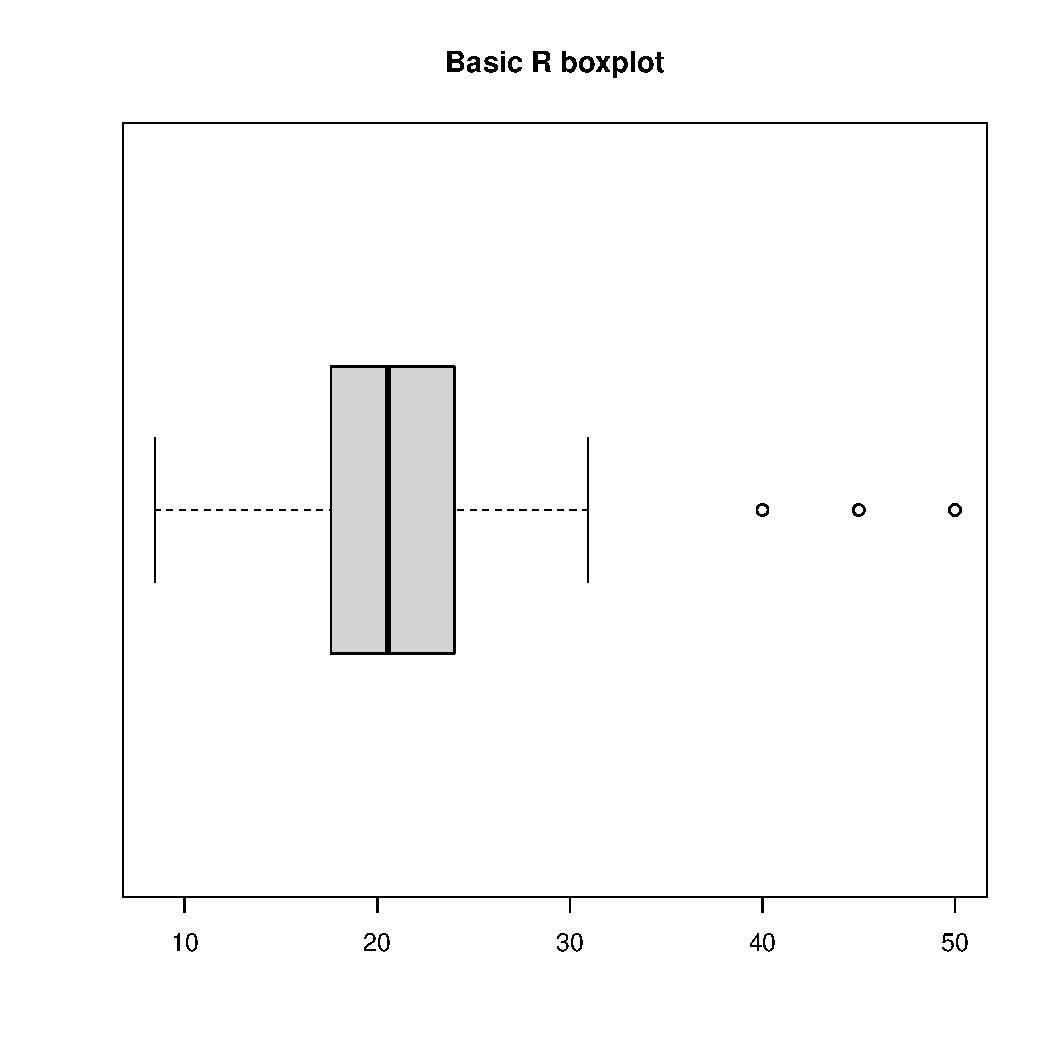
\includegraphics[width=\textwidth]{./images/boxplot.pdf}
    \caption{Boxplot}
    \label{boxplot}
  \end{minipage}
  \hfill  % This adds a space between the two figures
  \begin{minipage}[b]{0.45\textwidth}
    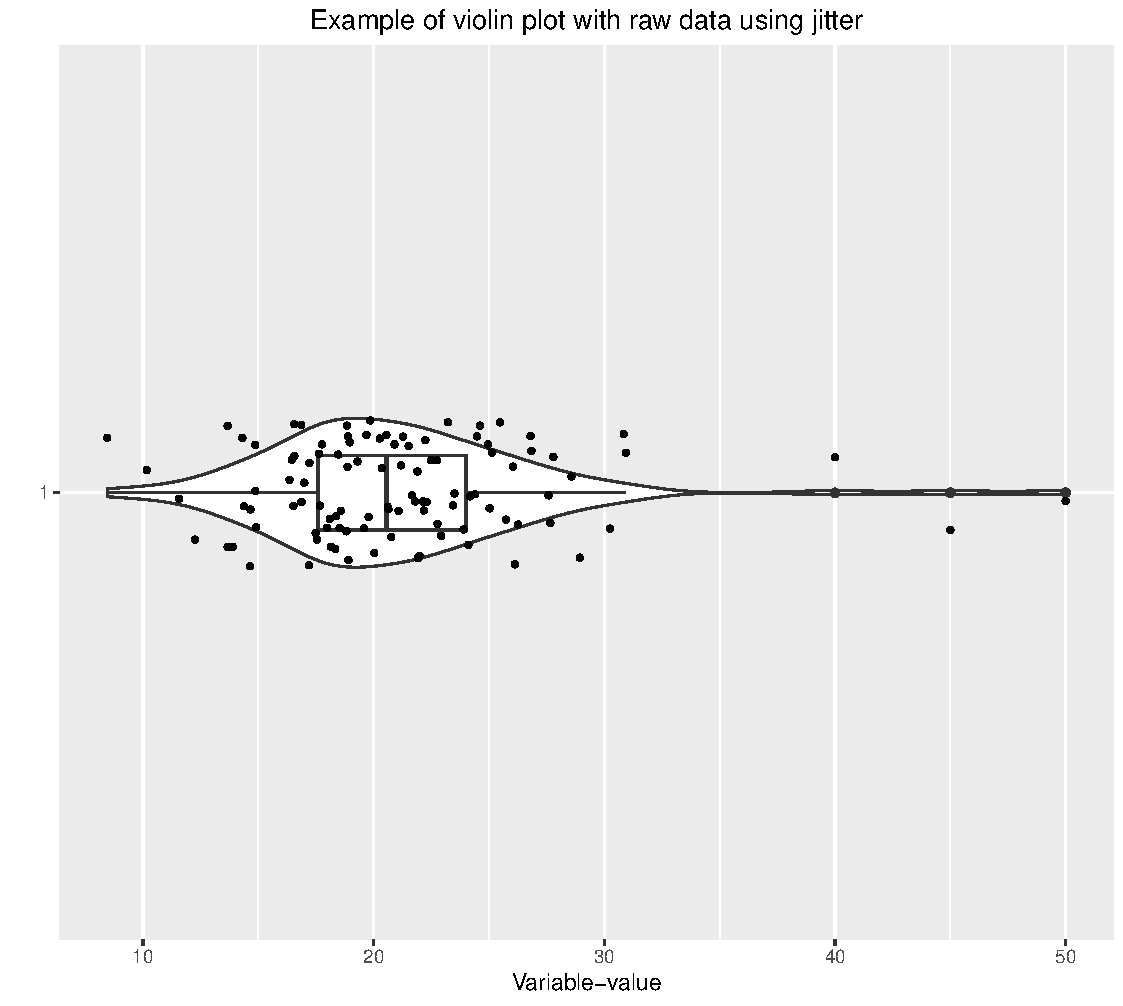
\includegraphics[width=\textwidth]{./images/violin_plot.pdf}
    \caption{Violin Plot}
    \label{violinplot}
  \end{minipage}
\end{figure}

\subsection{Histograms vs. density plots plus boxplots}
Especially for smaller sample sizes, a more informative boxplot is advised, see figures \ref{histogram} and \ref{densityplot}. This gives a richer impression of the data. Histograms and boxplots for small sample sizes are problematic.

\begin{figure}[htbp]
  \centering
  \begin{minipage}[b]{0.45\textwidth}
    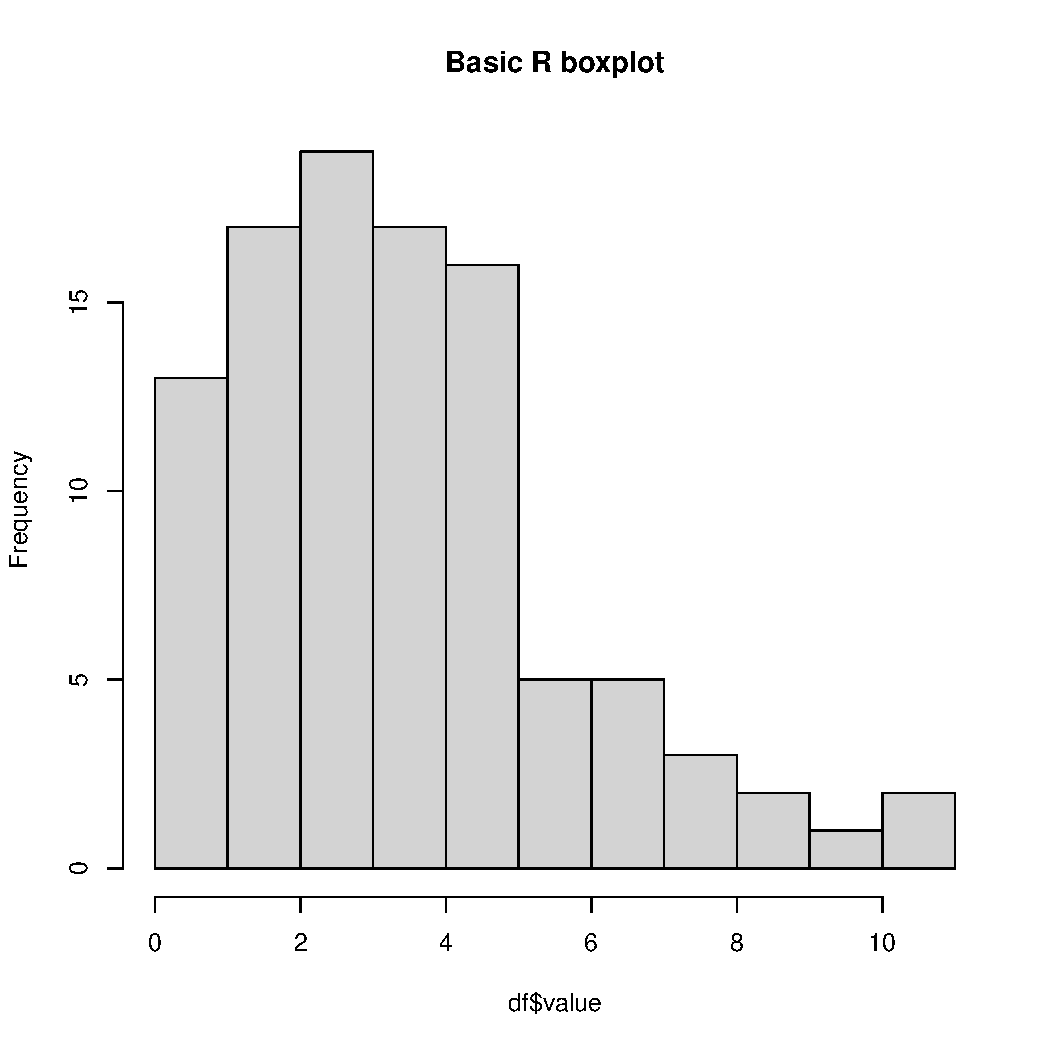
\includegraphics[width=\textwidth]{./images/histogram.pdf}
    \caption{Histogram}
    \label{histogram}
  \end{minipage}
  \hfill  % This adds a space between the two figures
  \begin{minipage}[b]{0.45\textwidth}
    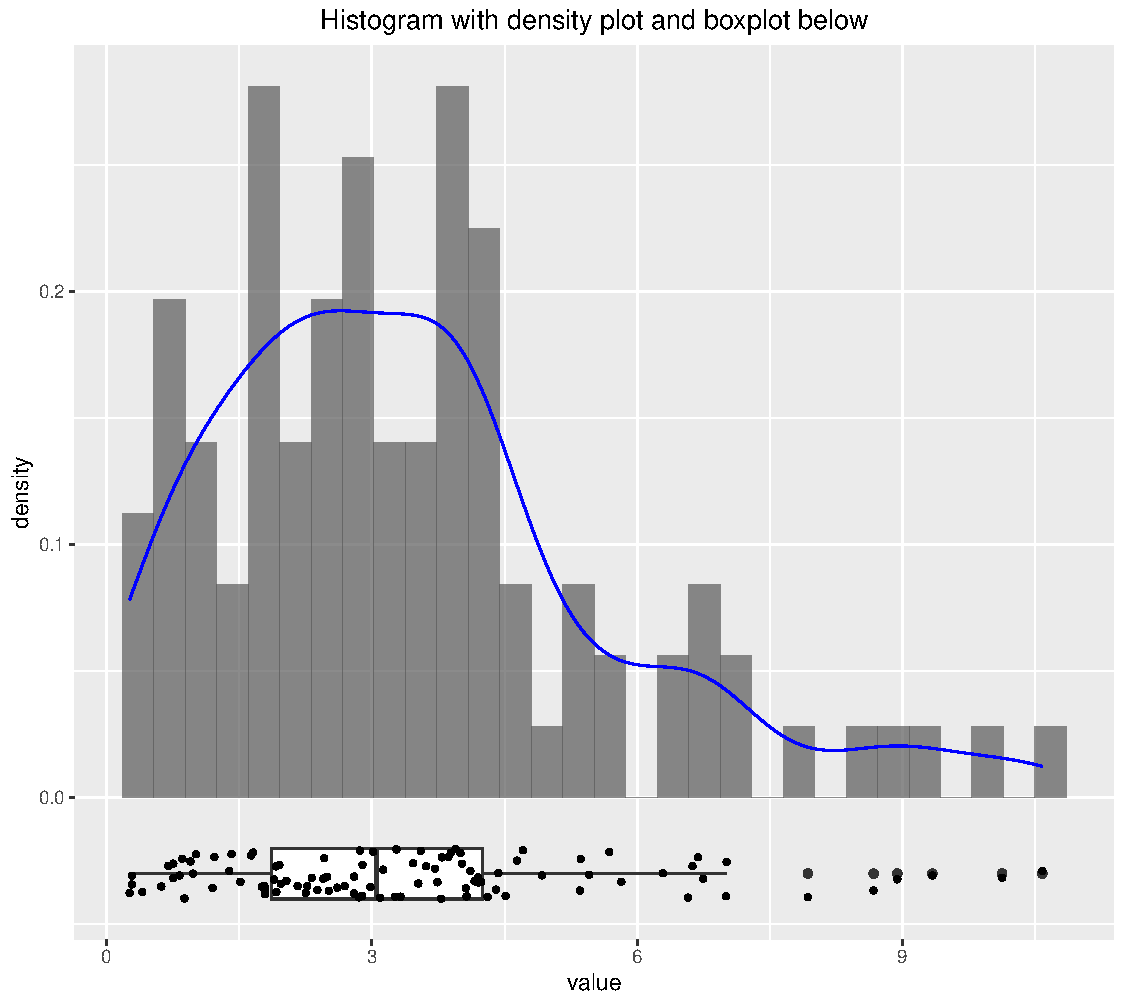
\includegraphics[width=\textwidth]{./images/density_plot_with_boxplot.pdf}
    \caption{Histogram and Boxplot}
    \label{densityplot}
  \end{minipage}
\end{figure}

\section{Missing values}
Do I have missing values in the data I want to analyze? If yes, how many in which variables?
Rule of thumb: if more than 3\% one should use imputation, one could use k-Nearst-Neighbour imputation for instance, which is fast and good \cite{VIM}.
Missing values can be visualized nicely using the package \textit{visdat} \cite{visdat} and the command \textit{vis\_miss()} - see figure \ref{fig:vismiss}. 

\begin{figure}[h!]
  \centering
  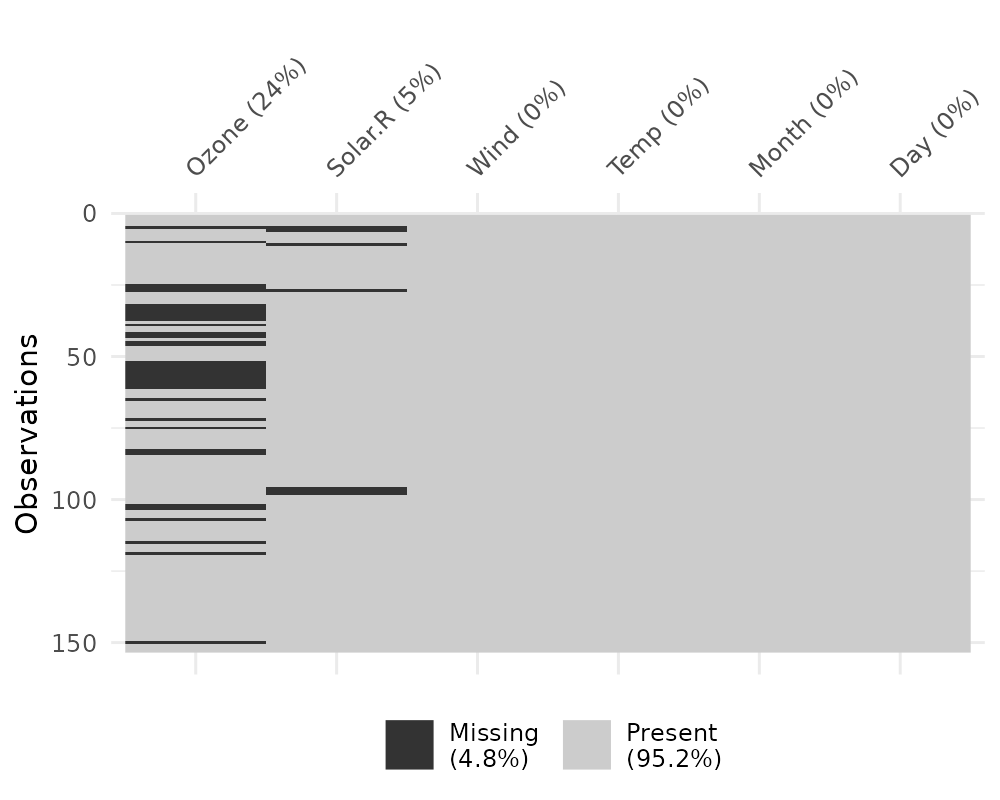
\includegraphics[width=0.5\textwidth]{./images/vis_miss.png}
  \caption{Visualization of missing values.}
  \label{fig:vismiss}
\end{figure}

\section{Model assumptions and assumptions for statistical tests}
Usually, every statistical model and test has assumptions that should be met if one wants to do inference statistics. It is important to check these assumptions. E.g., for a multiple regression model, one has to check linearity, homoscedasticity, influential points, normality of the residuals and more general: how does the model fit the data?
One could use the \textit{plot}-command on the regression-model object oder work with the package \textit{performance} 
For the popular \textit{t}-test one could check the normality of the mean (or the data itself, as is often done), and homogeneity of variances.

\section{Statistical modeling}
The goal is to estimate a model that fits the data well. There are many tutorials on which model or statistical test one should choose \cite{Parab2010ChoosingST} \cite{Abdi2023}. Among other aspects to consider, important are
\begin{itemize}
\item What type is the variable to be explained (Y): count data, percent data, continuous data, binary data (0/1)? Depending on this, different models are used.
\item What type of relationship is expected between the explanatory variables ($x_i$) and the outcome (Y) - linear, polynomial, exponential?
\item Which variables belong into the statistical model, what are potential confounders and how do I choose variables to include into the model (variable selection)? How were the variables pre-selected?
\item Does the model fit the data and are the model assumptions met reasonably well? 
\item What do I intend to do with the model? Do I want to explain relationships between variables (maybe even do causal inference?) or do I just want to predict an outcome as best as possible \cite{shmueli2010explain}?
\end{itemize}

In the future, there will be more and more Bayesian and causal modeling.

\section{Code availability}
Make all your analysis code and (if possible) data publicly available. You could for instance use github for posting code online. \href{https://osf.io/tf5xu/?view_only=}{Here}  is an example of a researcher sharing his code.

\newpage

\bibliographystyle{alpha}
%\bibliographystyle{plainnat}
%\bibliographystyle{unsrtnat}
\bibliography{references}


\end{document}


